\documentclass{article}
\usepackage{graphicx} % Required for inserting images

\usepackage{amsmath,amsfonts,amsthm,amssymb}
\usepackage{algorithmicx}
\usepackage{algorithm,algpseudocode}
\usepackage{multirow}

\newtheorem{prop}{Proposition}
\newtheorem{lem}{Lemma}
\newtheorem{thm}{Theorem}
\newtheorem{assu}{Assumption}

\newcommand{\simiid}{\overset{\text{i.i.d.}}{\sim}}
\newcommand{\limN}{\underset{N \rightarrow \infty}{\longrightarrow}}
\newcommand{\R}{\mathbb R}

\DeclareMathOperator{\prob}{P}
\DeclareMathOperator{\E}{E}
\DeclareMathOperator{\pred}{pred}
\DeclareMathOperator{\upd}{upd}
\DeclareMathOperator{\for}{for}

\bibliographystyle{elsarticle-num}

\title{Particle Approximation for Optimal Forecasting in State-Space Models}
\author{Paul Bui Quang}
\date{2020}

\begin{document}

\maketitle

\begin{abstract}
State-space models are statistical models for time series where observations are generated from a latent state process. Particle filtering is a well established sequential Monte Carlo algorithm to estimate the state given the observations in state-space models. We propose an extension of particle filtering, called particle forecasting, to estimate future data points given available observations. Particle forecasting computes forecasts in the form of empirical distributions. We review convergence results (almost surely and in mean squared error) of particle filtering and we obtain similar results for particle forecasting. Simulation experiments illustrate the convergence analysis. In the simulations, we use probability integral transform to assess the performance of distributional forecasts.
\end{abstract}

\section{Introduction}

\subsection{Context and Problem Statement}

Forecasting is an important task in statistics and machine learning, consisting in predicting future values of an observed time series. Many forecasting techniques are based on statistical modelling, involving models such as ARIMA, GARCH, or regression models \cite{Hyndman2018}.

State-space models are flexible statistical models where observations are generated from a dynamic latent state. They arise in many scientific fields, especially econometrics \cite{Taylor1986} and engineering \cite{BuiQuang2016,Gustafsson2002}. Inference problems in state-space models studied in the literature concern estimating the hidden state over time (filtering or smoothing), or estimating the static parameter identifying the model \cite{Cappe2005,Kantas2015,Sarkka2013}. 
Although they describe time series, forecasting in state-space models has not attracted much attention, outside the case where the observation process and the state process are linear with additive Gaussian noise \cite{Petris2009}.

We propose in this paper an algorithm to compute forecasts in general state-space models. This algorithm, called particle forecasting, is an extension of particle filtering (or sequential Monte Carlo method), which is a well established technique for state estimation in these models, based on importance sampling \cite{Arulampalam2002,Doucet2000,Doucet2011}. In particular, particle forecasting yields forecasts in the form of distributions rather than point values, which allows to assess prediction uncertainty \cite{Gneiting2014}.

In Section \ref{sec:dlm} below, we describe linear Gaussian state-space models, also called dynamic linear models. In Section \ref{sec:filter-forecast}, we define the model setup and the two inference problems we focus on: Bayesian filtering and optimal forecasting. The particle filter for Bayesian filtering and the particle forecast for optimal forecasting are presented in Section \ref{sec:particle-approx}. In Section \ref{sec:convergence}, we review convergence results of particle filtering and show the convergence of particle forecasting (almost surely and in mean squared error), using the same methodology as Crisan and Doucet in \cite{Crisan2002}, based on the description of the algorithms with measure-valued operators. Numerical experiments are presented in Section \ref{sec:numerical-xp}, where the quality of distribution forecasts is assessed with test-based procedures.

Throughout the article, the following notations are used:
\begin{itemize}
    \item $a_{0:t}$\,: sequence $\{a_0,a_1,\dots,a_t\}$,
    \item $\delta_a$\,: Dirac measure centered at $a$,
    \item $\displaystyle \int \phi \, \nu$\,: integral of $\phi$ w.r.t.\ the measure $\nu$,
    \item $\mathcal N(m,\sigma^2)$\,: Gaussian distribution with mean $m$ and variance $\sigma^2$,
    \item $\mathcal U(a,b)$\,: uniform distribution over the real segment $[a,b]$.
\end{itemize}

\subsection{Dynamic Linear Models}
\label{sec:dlm}

A dynamic linear model is a state-space model where the hidden (unobserved) state obeys to the linear discrete-time dynamics
\begin{equation*}
    X_t = F_t X_{t-1} + V_t
\end{equation*}
for $t \geq 1$ and $X_0 \sim \mathcal N(m_0, Q_0)$, where $\{V_t\}_t$ is a Gaussian white noise, and the observation process is also linear as
\begin{equation*}
    Y_t = H_t X_t + W_t
\end{equation*}
for $t \geq 0$, where $\{W_t\}_t$ is a Gaussian white noise.

In a dynamic linear model, filtering, smoothing and forecasting are optimally solved by the Kalman filter and its extensions \cite{Kalman1960,Petris2009}. We consider in this paper general state-space models, for example when the linear functions mapping $X_{t-1}$ to $X_t$ and $X_t$ to $Y_t$ above are replaced by nonlinear mappings.
placed by nonlinear mappings.

\section{Bayesian Filtering and Optimal Forecasting}
\label{sec:filter-forecast}

\subsection{Model Setup}

General state-space models, also called hidden Markov models, are stochastic processes composed of an unobserved process $\{X_t\}_t$, called the state process, and an observed process $\{Y_t\}_t$, called the observation process, where $\{X_t, Y_t\}_t$ is a discrete-time time Markov process such that
\begin{equation*}
    \prob[X_t \in dx_t, Y_t \in dy_t \mid X_{0:t-1}=x_{0:t-1}, Y_{0:t}=y_{0:t}] = Q_t(x_{t-1},dx_t) \, g_t(y_t \mid x_t) \, \lambda(dy_t)
\end{equation*}
for all $t \geq 1$ and $\prob[X_0 \in dx_0, Y_0 \in dy_0] = Q_0(dx_0) \, g_0(y_0 \mid x_0) \, \lambda(dy_0)$ \cite[Chapter 1]{Cappe2005}. The state process takes values in $\R^d$ equipped with its Borelian set $\mathcal B(\R^d)$; it is a Markov process with kernel $Q_t$. The observation process takes values in a measure space $(E, \mathcal Y, \lambda)$; $g_t(\cdot | x_t)$ is the conditional density of $Y_t$ given $X_t=x_t$ w.r.t.\ the dominating measure $\lambda$.

We use throughout the article the term "state-space model"  \cite{Petris2009,Sarkka2013} rather than the term "hidden Markov model" \cite{Cappe2005}. "State-space model" is more prevalent in the literature, especially on practical applications \cite{Gustafsson2002,Petris2009}. Besides "hidden Markov model" often specifically refers to models where the state process is a discrete Markov chain \cite{Rabiner1989}, whereas we consider continuous value state processes in this article.

One typical example of state-space model is the following:
\begin{align}
    X_t &= F_t(X_{t-1}) + V_t \label{eq:nonlinear-state} \\
    Y_t &= H_t(X_t) + W_t \label{eq:nonlinear-obs}
\end{align}
for $t \geq 1$ with initial condition $X_0 \sim Q_0$, where $\{V_t\}_t$ and $\{W_t\}_t$ are independent noise processes (non necessarily Gaussian) and $F_t$ and $H_t$ are nonlinear mappings. This is the nonlinear non-Gaussian version of the dynamic linear model in Section \ref{sec:dlm}.

Several statistical inference problems related to state-space models are addressed in the literature \cite{Cappe2005,Kantas2015,Sarkka2013}:
\begin{itemize}
    \item Parameter estimation: identifying the best data-generating process in a given parametric family. The parameter is static and is generally a vector. For example, in the model given by Equations \eqref{eq:nonlinear-state} and \eqref{eq:nonlinear-obs}, the parameter identifies the distributions of $V_t$ and $W_t$ and the mappings $F_t$ and $H_t$.
    %for example $\theta = (\alpha,\beta,\sigma)$ in the SV model above;
    \item Filtering: estimating sequentially at each time step the current hidden state $X_t$ given the available observations $Y_{0:t}$.
    \item Smoothing: estimating past hidden states $X_s$, where $s \leq t$, given observations $Y_{0:t}$.
\end{itemize}

In this paper, we address another inference problem, forecasting, defined as: estimating a future observation $Y_{t+h}$ given the available observations $Y_{0:t}$.

In practical applications, the model structure is often known up to an unknown parameter and one must estimate the parameter before performing other inference tasks (filtering, smoothing, forecasting). Parameter estimation can be done online (processing data points sequentially) or offline (processing the dataset as one batch), by likelihood maximization or Bayesian inference (see \cite{Kantas2015} for a comprehensive review). In this article, we address filtering and forecasting assuming that the model parameter, if any, is known or has been previously estimated.
\subsection{Bayesian Filtering}

Bayesian filtering consists in computing sequentially the conditional distribution of the current state $X_t$ and of the next state $X_{t+1}$ given the available observations $Y_{0:t}$ \cite{Cappe2005,Sarkka2013}.

Let the \textit{predictor} and the \textit{filter} respectively be the conditional distributions
\begin{equation*}
    \mu_{t \mid t-1}(dx_t) = \prob[X_t \in dx_t \mid Y_{0:t-1}]
\end{equation*}
and
\begin{equation*}
    \mu_t(dx_t) = \prob[X_t \in dx_t \mid Y_{0:t}]
\end{equation*}
at each time step $t \geq 0$ (with $\mu_{0 \mid -1} = Q_0$ by convention).

The predictor and the filter obey to a recursive relation that is conveniently written with measure-valued operators. The prediction operator is defined as
\begin{equation}
\label{eq:pred-operator}
    \pred_t(\nu) = \int Q_t(x,\cdot) \, \nu(dx)
\end{equation}
and the update operator as
\begin{equation}
\label{eq:upd-operator}
    \upd_t(\nu) = \frac{g_t(Y_t \mid \cdot) \, \nu(\cdot)}{\int g_t(Y_t \mid x) \, \nu(dx)}
\end{equation}
at each time $t \geq 0$, where $\nu$ is a probability measure. One then has the prediction step
\begin{equation*}
    \mu_{t \mid t-1} = \pred_t(\mu_{t-1})  
\end{equation*}
from the Chapman-Kolmogorov equation and the update step
\begin{equation*}
    \mu_t = \upd_t(\mu_{t \mid t-1})
\end{equation*}
from the Bayes formula.

\subsection{Optimal Forecasting}

Optimal forecasting consists in computing the conditional distribution of a future (non observed) data point $Y_{t+h}$, given the available observations $Y_{0:t}$, for some time horizon $h>0$.

Let the \textit{forecast} be the conditional distribution
\begin{equation*}
    f_{t+h \mid t}(dy_{t+h}) = \prob[Y_{t+h} \in dy_{t+h} \mid Y_{0:t}].
\end{equation*}
It is the "ideal forecast" in the terminology of Gneiting and Katzfuss \cite{Gneiting2014}.

Let
\begin{align*}
    Q_{t+1:t+h}(x_t,dx_{t+h}) =& \prob [X_{t+h} \in dx_{t+h} \mid X_t=x_t] \\
    =& \int_{\{x_{t+h-1}  \in \R^d\}} \cdots \int_{\{x_{t+1} \in \R^d\}} Q_{t+h}(x_{t+h-1},dx_{t+h}) \times \cdots \times Q_{t+1}(x_t,dx_{t+1}) \\
    =& \int_{\{x_{t+h-1} \in \R^d\}} Q_{t+h}(x_{t+h-1},dx_{t+h}) \cdots \int_{\{x_{t+1} \in \R^d\}} Q_{t+1}(x_t,dx_{t+1})
\end{align*}
and let
\begin{equation*}
    \pred_{t+1:t+h} = \pred_{t+h} \circ \cdots \circ \pred_{t+1}.
\end{equation*}
be the composition product of the prediction operators from time $t+1$ to time $t+h$, so that
\begin{equation}
\label{eq:compo-pred}
    \pred_{t+1:t+h}(\nu) = \int Q_{t+1:t+h}(x,\cdot) \, \nu(dx). 
\end{equation}

Let the \textit{state forecast} be the conditional distribution
\begin{equation*}
    \mu_{t+h \mid t}(dx_{t+h}) = \prob [X_{t+h} \in dx_{t+h} \mid Y_{0:t}].
\end{equation*}
One has that
\begin{equation*}
    \mu_{t+h \mid t}(dx_{t+h}) = \int_{\{x_t \in \R^d\}} Q_{t+1:t+h}(x_t,dx_{t+h}) \, \mu_t(dx_t),
\end{equation*}
that is
\begin{equation*}
    \mu_{t+h \mid t} = \pred_{t+1:t+h} (\mu_t).
\end{equation*}

Besides, let the forecast operator be the measure-valued mapping defined as
\begin{equation}
\label{eq:for-operator}
    \for_{t+h}(\nu) = [\int g_{t+h}(\cdot | x) \, \nu(dx)] \, \lambda(\cdot).
\end{equation}
The forecast verifies
\begin{align*}
    f_{t+h \mid t}(dy_{t+h}) &= \prob[Y_{t+h} \in dy_{t+h} \mid Y_{0:t}] \\
    &= \int_{\{x_{t+h} \in \R^d\}} \prob[Y_{t+h} \in dy_{t+h} \mid X_{t+h} = x_{t+h}] \, \prob[X_{t+h} \in dx_{t+h} \mid Y_{0:t}] \\
    &= [\int g_{t+h}(y_{t+h} \mid x_{t+h}) \, \mu_{t+h \mid t}(dx_{t+h})] \, \lambda(dy_{t+h}),
\end{align*}
so that
\begin{equation*}
    f_{t+h \mid t} = \for_{t+h}(\mu_{t+h \mid t}) = \for_{t+h}(\pred_{t+1:t+h} (\mu_t)).
\end{equation*}


\section{Particle Filtering and Particle Forecasting}
\label{sec:particle-approx}

Particle filtering (for Bayesian filtering) and particle forecasting (for optimal forecasting) are described in this section. Particle filters, also called sequential Monte Carlo methods, are algorithms based on importance sampling that recursively approximate the filter and the predictor. Several tutorial articles on particle filtering are available \cite{Arulampalam2002,Cappe2007,Doucet2000,Doucet2011}. The first version of particle filter has been proposed by Gordon et al.\ in \cite{Gordon1993}. Particle forecasting is an extension of particle filtering, which we propose in this paper as a novel sequential Monte Carlo method to approximate the optimal forecast.

\subsection{Particle Filtering}

Particle filtering consists in approximating the predictor and the filter recursively by a weighted sum of Dirac measures.

At initial time $t=0$, the predictor is $\mu_{0 \mid -1} = Q_0$. One generates an i.i.d.\ sample $\xi^1_0,\dots,\xi^N_0$ of random vectors (called particles) in $\R^d$ from $Q_0$. The particle approximation of the predictor is the empirical measure
\begin{equation*}
    \mu^N_{0 \mid -1} = \frac 1N \sum_{i=1}^N \delta_{\xi^i_0}.
\end{equation*}

The observation $Y_0$ is then used through the update operator defined in Equation \eqref{eq:upd-operator}. The particle approximation of the filter is
\begin{equation*}
    \mu^N_0 = \upd_0(\mu^N_{0 \mid -1}) = \frac{\sum_{i=1}^N g_0(Y_0 \mid \xi^i_0) \, \delta_{\xi^i_0}}{\sum_{i=1}^N g_0(Y_0 \mid \xi^i_0)} = \sum_{i=1}^N w^i_0 \, \delta_{\xi^i_0}
\end{equation*}
where the weights are $\displaystyle w^i_0 = \frac{g_0(Y_0 \mid \xi^i_0)}{\sum_{i=1}^N g_0(Y_0 \mid \xi^i_0)}$ for all $i \in \{1,\dots,N\}$ (so they sum up to one). Thus $\mu^N_0$ is obtained by importance sampling, with a sampling step and a weighting step.

Suppose now one has an approximation $\mu^N_{t-1}$ of the filter at time $t-1 \geq 0$ as
\begin{equation*}
    \mu^N_{t-1} = \sum_{i=1}^N w^i_{t-1} \, \delta_{\xi^i_{t-1}}.
\end{equation*}
By applying the prediction operator defined in Equation \eqref{eq:pred-operator} to $\mu^N_{t-1}$, one gets a mixture distribution
\begin{equation}
\label{eq:pred-PF}
    \pred_t(\mu^N_{t-1}) = \int Q_t \, \mu^N_{t-1}  = \sum_{i=1}^N w^i_{t-1} \, Q_t(\xi^i_{t-1},\cdot).
\end{equation}
The approximation $\mu^N_{t \mid t-1}$ of the predictor is obtained by drawing a sample of new particles from this mixture distribution, independently given $\xi^1_{t-1},\dots,\xi^N_{t-1}$. In practice, the new particles $\xi^1_t,\dots,\xi^N_t$ are generated by repeating the two following steps for all $i \in \{1,\dots,N\}$:
\begin{itemize}
    \item[Selection] Draw an index $j \in \{1,\dots,N\}$ where the drawing probabilities are the weights $w^1_{t-1},\dots,w^N_{t-1}$, i.e.\ draw $j$ from the Multinomial distribution over $\{1,\dots,N\}$ with parameters $w^1_{t-1},\dots,w^N_{t-1}$.
    \item[Propagation] Generate $\xi^i_t$ from the distribution $Q_t(\xi^j_{t-1},\cdot)$, i.e.\ the mixture component corresponding to the selected index.
\end{itemize}
The particle approximation of the predictor is then
\begin{equation*}
    \mu^N_{t \mid t-1} = \sum_{i=1}^N w^i_{t-1} \, \delta_{\xi^i_t}
\end{equation*}
where $\xi^1_t,\dots,\xi^N_t \mid (\xi^1_{t-1},\dots,\xi^N_{t-1}) \simiid \pred_t(\mu^N_{t-1})$.

The particle approximation of the filter is obtained by updating the predictor approximation. Applying the update operator to $\mu^N_{t \mid t-1}$ yields
\begin{equation*}
    \mu^N_t = \upd_t(\mu^N_{t \mid t-1}) = \sum_{i=1}^N w^i_t \, \delta_{\xi^i_t},
\end{equation*}
where the new weights are $\displaystyle w^i_t = \frac{g_t(Y_t \mid \xi^i_t)}{\sum_{i=1}^N g_t(Y_t \mid \xi^i_t)}$ for all $i \in \{1,\dots,N\}$.

The particle filter is summarized in Algorithm \ref{algo:pf}. This version corresponds to the seminal algorithm proposed by Gordon et al.\ in \cite{Gordon1993} and is also referred to as the bootstrap filter.

In the bootstrap filter, the particle sampling mechanism is given by the Markov kernel $Q_t$ from the state process. It is possible to use a different sampling distribution, denoted $\tilde Q_t$, as soon as the derivative (in the Radon-Nikodym sense) $\tilde g_t(x_{t-1},\cdot) = \displaystyle \frac{dQ_t(x_{t-1},\cdot)}{d\tilde Q_t(x_{t-1},\cdot)}$ exists for all $x_{t-1} \in \R^d$. In this case, the particles are sampled as $\displaystyle \xi^i_t \sim \tilde Q_t(\xi^i_{t-1},\cdot)$ and the weights are computed as $\displaystyle w^i_t = \frac{g_t(\xi^i_t) \, \tilde g_t(\xi^i_{t-1},\xi^i_t)}{\sum_{i=1}^N g_t(\xi^i_t) \, \tilde g_t(\xi^i_{t-1},\xi^i_t)}$ for all $i \in \{1,\dots,N\}$. Although choosing $Q_t$ is practically simpler, using a different sampling kernel $\tilde Q_t$ in the propagation step can lead to lower weight variance and better algorithm performance \cite{Cappe2007, Doucet2000, Doucet2011}.

The resampling step is necessary to avoid particle degeneracy. Without resampling, after some time most particles get a zero weight and only a few particles get a significant weight. This impoverishment of particle weights drastically degrades particle approximations. However it is not necessary in practice to perform resampling at each time step. Resampling is generally done according to a criterion monitoring the quality of the particle sample, for example when the effective sample size $\displaystyle N_\text{eff} = \frac{1}{\sum_{i=1}^N (w^i_t)^2}$ falls below a preset threshold.

\begin{algorithm}
\caption{Particle Filter}
\label{algo:pf}
\begin{algorithmic}
  \State observe $Y_0$
  \For {$i=1 \cdots N$}
    \State sample $\xi^i_0 \sim Q_0$
    \State compute $w^i_0 \propto g_0(Y_0 \mid \xi^i_0)$
  \EndFor
  \State normalize weights
  \State set $t$ to $1$
  \Loop
    \State observe $Y_t$
    \For{$i = 1 \cdots N$}
      \State sample $j \sim \operatorname{Multinomial}(\{1,\dots,N\}, \{w^1_{t-1},\dots,w^N_{t-1}\})$ \Comment{selection}
      \State sample $\xi^i_t \sim Q_t(\cdot \mid \xi^j_{t-1})$ \Comment{propagation}
      %\State observe $Y_t$
      \State compute $w^i_t \propto g_t(Y_t \mid \xi^i_t)$ \Comment{weighting}
    \EndFor
    \State normalize weights
    \State increment $t$
  \EndLoop
\end{algorithmic}
\end{algorithm}

\subsection{Particle Forecasting}

The algorithm proposed in this article approximates the forecast (conditional distribution of the future data point $Y_{t+h}$ given the available observations $Y_{0:t}$) and the state forecast (conditional distribution of $X_{t+h}$ given $Y_{0:t}$) defined in Section \ref{sec:filter-forecast}. The particle forecast is run after the particle filter and uses the current weights and particles at time $t$.

Suppose one has the approximation $\mu^N_t$ of the filter at time $t$ given by the particle filter in Algorithm \ref{algo:pf}.

By applying the composition product of prediction operators defined in Equation \eqref{eq:compo-pred}, one gets
\begin{equation}
\label{eq:pred-PFor}
    \pred_{t+1:t+h}(\mu^N_t) = \sum_{i=1}^N w^i_t \, Q_{t+1:t+h}(\xi^i_t,\cdot).
\end{equation}
It is a mixture distribution, as in Equation \eqref{eq:pred-PF} for the particle filter. The approximation $\mu^N_{t+h \mid t}$ of the state forecast is obtained by sampling from this distribution independently given $\xi^1_t,\dots,\xi^N_t$. Like in particle filtering, this is done by repeating $N$ times a selection step and a propagation step. Here, after an index $j \in \{1,\dots,N\}$ is selected according to the weights $w^1_t,\dots,w^N_t$, a new particle is generated by propagating $h$ steps ahead the selected particle $\xi^j_t$. In practice, one draws from the distribution $Q_{t+1:t+h}(\xi^j_t,\cdot)$ by recursively generating new particles using the Markov kernel from time $t+1$ to time $t+h$. The particle approximation of the state forecast is then
\begin{equation*}
    \mu^N_{t+h \mid t} = \frac 1N \sum_{i=1} \delta_{\xi^i_{t+h \mid t}}
\end{equation*}
where $\xi^1_{t+h \mid t},\dots,\xi^N_{t+h \mid t} \mid (\xi^1_t,\dots,\xi^N_t) \simiid \pred_{t+1:t+h}(\mu^N_t)$.

Then, by applying the forecast operator defined in Equation \eqref{eq:for-operator} to $\mu^N_{t+h \mid t}$, one gets
\begin{equation}
\label{eq:forecast-PFor}
    \for_{t+h}(\mu^N_{t+h \mid t}) = \frac 1N \sum_{i=1} g_{t+h}(\cdot \mid \xi^i_{t+h \mid t}) \, \lambda(\cdot).
\end{equation}
It is again a mixture distribution. To generate from this mixture, an index $j \in \{1,\dots,N\}$ is randomly selected with probability $1/N$ and one draws from the corresponding mixture component $g_{t+h}(\cdot \mid \xi^j_{t+h}) \, \lambda(\cdot)$. The particle approximation of the forecast is then
\begin{equation*}
    f^N_{t+h \mid t} = \frac 1N \sum_{i=1} \delta_{\zeta^i_{t+h \mid t}}
\end{equation*}
where $\zeta^1_{t+h \mid t},\dots,\zeta^N_{t+h \mid t} \mid (\xi^1_{t+h \mid t},\cdots,\xi^N_{t+h \mid t}) \simiid \for_{t+h}(\mu^N_{t+h \mid t})$.

Particle forecasting is thus based on the same algorithmic ideas as particle filtering. It is summarized in Algorithm \ref{algo:forecast}.

\begin{algorithm}
\caption{Particle Forecast}
\label{algo:forecast}
\begin{algorithmic}
  \For{$i = 1 \cdots N$}
      \State sample $j \sim \operatorname{Multinomial}(\{1,\dots,N\}, \{w^1_t,\dots,w^N_t\})$
      \State sample $\xi^i_{t+1 \mid t} \sim Q_{t+1}(\xi^j_t,\cdot)$
    \For{$s = 2 \cdots h$}
      \State sample $\xi^i_{t+s \mid t} \sim Q_{t+s}(\xi^i_{t+s-1 \mid t},\cdot)$
    \EndFor
  \EndFor
  \For{$i = 1 \cdots N$}
    \State sample $j \sim \operatorname{Multinomial}(\{1,\dots,N\}, \{1/N,\dots,1/N\})$
    \State sample $\zeta^i_{t+h \mid t} \sim g_{t+h}(\cdot \mid \xi^j_{t+h \mid t}) \, \lambda(\cdot)$
  \EndFor
\end{algorithmic}
\end{algorithm}

\section{Convergence Analysis}
\label{sec:convergence}

First results on the convergence of particle filtering were obtained by Del Moral in \cite{DelMoral1996,DelMoral1998}. An analysis of the algorithm with randomly selected resampling times has been provided by Douc and Moulines in \cite{Douc2008}. In \cite{Crisan2002}, Crisan and Doucet present convergence results based on a description of particle filtering with continuous measure-valued operators. We follow a similar approach in this article to review results for particle filtering and extend them to particle forecasting. We address almost sure convergence and convergence in mean squared error in the weak topology of probability measures \cite[Chapter 2]{Huber1981}. In this topology, a sequence of probability measures $\{\lambda_n\}_n$ tends to $\lambda$ if $\displaystyle \int \phi(x) \, \lambda_n(dx)$ tends to $\displaystyle \int \phi(x) \, \lambda(dx)$ for all continuous bounded function $\phi$.

\subsection{Sampling Operator}

Particle filtering and particle forecasting involve sampling from random probability measures.

Let $\nu^N(V_{1:N})$ by a random measure determined by a random vector $V_{1:N}=(V_1,\dots,V_N)$, i.e.
$$ \E[\int \phi \, \nu^N(V_{1:N}) \mid V_{1:N}] = \int \phi \, \nu^N(V_{1:N})$$
for all continuous bounded function $\phi$. The sampling operator $s^N$ maps $\nu^N(V_{1:N})$ to an empirical measure given by a sample $U_1,\dots,U_N$ from $\nu^N(V_{1:N})$, such that $U_i$ and $U_j$ are conditionally independent given $V_{1:N}$ for all $i \neq j$. That is
$$s^N(\nu^N(V_{1:N})) = \frac 1N \sum_{i=1}^N \delta_{U_i} \text{\ \ where\ } U_1,\dots,U_N \mid V_{1:N} \simiid \nu^N(V_{1:N}).$$

In particle filtering, the distribution $\pred_t(\mu^N_{t-1})$ in Equation \eqref{eq:pred-PF} is a random measure determined by $(\xi^1_{t-1},\dots,\xi^N_{t-1})$, hence it is in the form over which $s^N$ applies. Drawing particles as $$\xi^1_t,\dots,\xi^N_t \mid (\xi^1_{t-1},\dots,\xi^N_{t-1}) \simiid \pred_t(\mu^N_{t-1})$$
to approximate the predictor $\mu^N_{t \mid t-1}$ is formalized as applying $s^N$ to $\pred_t(\mu^N_{t-1})$, so that one has
$$ \mu^N_{t \mid t-1} = s^N(\pred_t(\mu^N_{t-1})).$$

In particle forecasting, the distributions $\pred_{t+1:t+h}(\mu^N_t)$ in Equation \eqref{eq:pred-PFor} and $\for_{t+h}(\mu^N_{t+h \mid t})$ in Equation \eqref{eq:forecast-PFor} are also random measures respectively determined by the random vectors $(\xi^1_t,\dots,\xi^N_t)$ and $(\xi^1_{t+h \mid t},\cdots,\xi^N_{t+h \mid t})$. Drawing
$$\xi^1_{t+h \mid t},\dots,\xi^N_{t+h \mid t} \mid (\xi^1_t,\dots,\xi^N_t) \simiid \pred_{t+1:t+h}(\mu^N_t),$$
to approximate the state forecast $\mu_{t+h \mid t}$, is formalized as
$$ \mu^N_{t+h \mid t} = s^N(\pred_{t+1:t+h}(\mu^N_t))$$
and drawing
$$ \zeta^1_{t+h \mid t},\dots,\zeta^N_{t+h \mid t} \mid (\xi^1_{t+h \mid t},\cdots,\xi^N_{t+h \mid t}) \simiid \for_{t+h}(\mu^N_{t+h \mid t}), $$
to approximate the forecast $f_{t+h \mid t}$, as
$$ f^N_{t+h \mid t} = s^N(\for_{t+h}(\mu^N_{t+h \mid t})).$$

Thus, Bayesian filtering and its particle approximation can be schematized as
\begin{equation*}
    \mu_{t-1} \, \overset{\pred_t}{\longrightarrow} \, \mu_{t \mid t-1} \, \overset{\upd_t}{\longrightarrow} \, \mu_t
\end{equation*}
\begin{equation*}
    \mu^N_{t-1} \, \overset{s^N \circ \, \pred_t}{\longrightarrow} \, \mu^N_{t \mid t-1} \, \overset{\upd_t}{\longrightarrow} \, \mu^N_t,
\end{equation*}
and optimal forecasting and its particle approximation can be schematized as
\begin{equation*}
    \mu_t \, \overset{\pred_{t+1:t+h}}{\longrightarrow} \, \mu_{t+h \mid t} \, \overset{\for_{t+h}}{\longrightarrow} \, f_{t+h \mid t}
\end{equation*}
\begin{equation*}
    \mu^N_t \, \overset{s^N \circ \, \pred_{t+1:t+h}}{\longrightarrow} \, \mu^N_{t+h \mid t} \, \overset{s^N \circ \, \for_{t+h}}{\longrightarrow} \, f^N_{t+h \mid t}.
\end{equation*}

The two following lemmas hold for the random probability measure $\nu^N(V_{1:N})$ and the sampling operator $s^N$ defined above. Their proofs are provided in Appendix \ref{sec:proof-sampling}.

\begin{lem} \label{lem:cv_sampling}
    For all continuous bounded function $\phi$, if
    $$\int \phi \, \nu^N(V_{1:N}) \limN \int \phi \, \nu \text{\ \ almost surely},$$
    then
    $$\int \phi \, s^N(\nu^N(V_{1:N})) \limN \int \phi \, \nu \text{\ \ almost surely.}$$
\end{lem}

\begin{lem} \label{lem:cv_sampling_l2}
    For all continuous bounded function $\phi$ and positive real number $m$, if
    $$\E[(\int \phi \, \nu^N(V_{1:N}) - \int \phi \, \nu)^2] \leq \frac{m}{N},$$
    then
    $$\E[(\int \phi \, s^N(\nu^N(V_{1:N})) - \int \phi \, \nu)^2] \leq \frac{(\sqrt{m} + \sqrt 2 |\sup \phi|)^2}{N}.$$
\end{lem}

\subsection{Convergence of Particle Filtering}

The almost sure convergence and the convergence in mean squared error, in the weak topology, of particle filtering can be established under Assumptions \ref{assu:feller} and \ref{assu:g_bounded} below \cite{Crisan2002}.

\begin{assu}\label{assu:feller}
  For all $t \geq 0$ and for all continuous bounded function $\phi$, the mapping $\displaystyle x_{t-1} \longmapsto \int \phi(x_t) \, Q_t(x_{t-1},dx_t)$ is continuous and bounded.
\end{assu}

\begin{assu}\label{assu:g_bounded}
  For all $t \geq 0$, $g_t(y \mid \cdot)$ is continuous, bounded and strictly positive for all $y$ ($\lambda$ almost surely).
\end{assu}

For example, consider the state process
\begin{equation*}
    X_t = F_t(X_{t-1}) + V_t
\end{equation*}
for $t \geq 1$ where $\{V_t\}_t \simiid \mathcal N(0,\sigma_v^2)$ (and $X_0 \sim Q_0$). If the mapping $F_t$ is continuous, then
\begin{equation*}
    \int \phi(x_t) \, Q_t(x_{t-1},dx_t) = \frac{1}{\sqrt{2\pi} \sigma_v} \int \phi(x_t) \, e^{-\frac{1}{2\sigma_v^2}(x_t-F_t(x_{t-1}))^2} \, dx_t
\end{equation*}
is continuous w.r.t.\ $x_{t-1}$ and Assumption \ref{assu:feller} is verified.

Now consider the observation process
\begin{equation}
\label{eq:obs_process}
    Y_t = H_t(X_t) + W_t
\end{equation}
for $t \geq 0$ where $\{W_t\}_t \simiid \mathcal N(0,\sigma_w^2)$. If the mapping $H_t$ is continuous, then
\begin{equation*}
    g_t(y \mid x) = \frac{1}{\sqrt{2\pi} \sigma_w} e^{-\frac{1}{2\sigma_w^2}(y-H_t(x))^2}
\end{equation*}
verifies Assumption \ref{assu:g_bounded}.

Under Assumptions \ref{assu:feller} and \ref{assu:g_bounded}, the measure-valued operators for prediction and update in Bayesian filtering, defined in Equations \eqref{eq:pred-operator} and \eqref{eq:upd-operator}, are continuous.

\begin{prop}\label{prop:pred_continuous}
    Under Assumption \ref{assu:feller}, the prediction operator $\pred_t$ is continuous in the weak topology.
\end{prop}

\begin{prop}\label{prop:upd_continuous}
    Under Assumption \ref{assu:g_bounded}, the update operator $\upd_t$ is continuous in the weak topology.
\end{prop}

The proofs of Propositions \ref{prop:pred_continuous} and \ref{prop:upd_continuous} are provided in Appendix \ref{sec:proof-continuity}.

The convergence of particle filtering is stated in Theorems \ref{thm:cv_filter} and \ref{thm:cv_filter_l2} below.

\begin{thm}\label{thm:cv_filter}
    Under Assumptions \ref{assu:feller} and \ref{assu:g_bounded}, for all continuous bounded function $\phi$,
    $$\int \phi \, \mu^N_{t \mid t-1} \limN \int \phi \, \mu_{t \mid t-1} \text{\ \ almost surely}$$
    and
    $$\int \phi \, \mu^N_t \limN \int \phi \, \mu_t \text{\ \ almost surely.}$$
\end{thm}

\begin{proof}
    At initial time, one has that $\displaystyle \mu^N_{0 \mid -1} = \frac 1N \sum_{i=1}^N \delta_{\xi^i_0}$ where $\xi^1_0,\dots,\xi^N_0 \simiid \mu_{0 \mid -1}$ ($\mu_{0 \mid -1} = Q_0$ by convention). Then $\displaystyle \int \phi \, \mu^N_{0 \mid -1} \limN \int \phi \, \mu_{0 \mid -1}$ almost surely according to the strong law of large numbers. The operator $\upd_0$ is continuous according to Proposition \ref{prop:upd_continuous} and $\mu^N_0 = \upd_0(\mu^N_{0 \mid -1})$, hence $\displaystyle \int \phi \, \mu^N_0 \limN \int \phi \, \mu_0$ almost surely.
    
    Let $t \geq 1$. Suppose that $\displaystyle \int \phi \, \mu^N_{t-1} \limN \int \phi \, \mu_{t-1}$ almost surely. The operator $\pred_t$ is continuous according to Proposition \ref{prop:pred_continuous}, then $\displaystyle \int \phi \, \pred_t(\mu^N_{t-1}) \limN \int \phi \, \pred_t(\mu_{t-1})$ almost surely. Since $\mu^N_{t \mid t-1} = s^N(\pred_t(\mu^N_{t-1}))$, then Lemma \ref{lem:cv_sampling} yields $\displaystyle \int \phi \, \mu^N_{t \mid t-1} \limN \int \phi \, \mu_{t \mid t-1}$ almost surely.
    
    The operator $\upd_t$ is continuous according to Proposition \ref{prop:upd_continuous} and $\mu^N_t = \upd_t(\mu^N_{t \mid t-1})$, then $\displaystyle \int \phi \, \mu^N_t \limN \int \phi \, \mu_t$ almost surely.
\end{proof}

\begin{thm}\label{thm:cv_filter_l2}
    Under Assumptions \ref{assu:feller} and \ref{assu:g_bounded}, for all continuous bounded function $\phi$, there exists positive real numbers $m_{t|t-1}(\phi)$ and $m_t(\phi)$ such that
    $$\E[(\int \phi \, \mu^N_{t \mid t-1} - \int \phi \, \mu_{t \mid t-1})^2] \leq \frac{m_{t|t-1}(\phi)}{N}$$
    and
    $$\E[(\int \phi \, \mu^N_t - \int \phi \, \mu_t)^2] \leq \frac{m_t(\phi)}{N}.$$
\end{thm}

\begin{proof}
    At initial time, one has that $\displaystyle \mu_0 = \frac{g_0 \, Q_0}{\int g_0 \, Q_0}$ and $\displaystyle \mu^N_0 = \frac{g_0 \, s^N(Q_0)}{\int g_0 \, s^N(Q_0)}$. Then
    \begin{align*}
        \frac{\int \phi \, g_0 \, s^N(Q_0)}{\int g_0 \, s^N(Q_0)} - \frac{\int \phi \, g_0 \, Q_0}{\int g_0 \, Q_0} = & \, \frac{\int \phi \, g_0 \, s^N(Q_0) - \int \phi \, g_0 \, Q_0}{\int g_0 \, Q_0} \\
        &- \frac{\int \phi \, g_0 \, s^N(Q_0)}{\int g_0 \, s^N(Q_0)} \times \frac{\int g_0 \, s^N(Q_0) - \int g_0 \, Q_0}{\int g_0 \, Q_0}.
    \end{align*}
    Hence
    \begin{multline*}
        \E[(\frac{\int \phi \, g_0 \, s^N(Q_0)}{\int g_0 \, s^N(Q_0)} - \frac{\int \phi \, g_0 \, Q_0}{\int g_0 \, Q_0})^2]^{1/2} \leq \E[(\frac{\int \phi \, g_0 \, s^N(Q_0) - \int \phi \, g_0 \, Q_0}{\int g_0 \, Q_0})^2]^{1/2} \\
        + \E[(\frac{\int \phi \, g_0 \, s^N(Q_0)}{\int g_0 \, s^N(Q_0)} \times \frac{\int g_0 \, s^N(Q_0) - \int g_0 \, Q_0}{\int g_0 \, Q_0})^2]^{1/2}
    \end{multline*}
    according to the Minkowski inequality, where the first term of the right-hand side verifies
    \begin{equation*}
        \E[(\frac{\int \phi \, g_0 \, s^N(Q_0) - \int \phi \, g_0 \, Q_0}{\int g_0 \, Q_0})^2] = \frac 1N \frac{\int \phi^2 \, g_0^2 \, Q_0 - (\int \phi \, g_0 \, Q_0)^2}{(\int g_0 \, Q_0)^2}
    \end{equation*}
    and the second term verifies
    \begin{align*}
        \E[(\frac{\int \phi \, g_0 \, s^N(Q_0)}{\int g_0 \, s^N(Q_0)} \times \frac{\int g_0 \, s^N(Q_0) - \int g_0 \, Q_0}{\int g_0 \, Q_0})^2] &\leq (\sup \phi)^2 \, \E[(\frac{\int g_0 \, s^N(Q_0) - \int g_0 \, Q_0}{\int g_0 \, Q_0})^2] \\
        &= \frac{(\sup \phi)^2}{N} \, \frac{\int g_0^2 \, Q_0 - (\int g_0 \, Q_0)^2}{(\int g_0 \, Q_0)^2}
    \end{align*}
    as $\displaystyle \int g_0 \, s^N(Q_0) = \frac 1N \sum_{i=1}^N g_0(Y_0 \mid \xi^i_0)$ where $\xi^1_0,\dots,\xi^N_0 \simiid Q_0$.

    Let $t \geq 1$. Suppose that $\displaystyle \E[(\int \phi \, \mu^N_{t-1} - \int \phi \, \mu_{t-1})^2] \leq \frac{m_{t-1}(\phi)}{N}$ for all continuous bounded function $\phi$. Then
    \begin{align*}
        & \E[(\int \phi \, [\int Q_t \, \mu^N_{t-1}] - \int \phi \, [\int Q_t \, \mu_{t-1}])^2] \\
        & = \E[(\int [\int \phi \, Q_t] \, \mu^N_{t-1} - \int [\int \phi \, Q_t ] \, \mu_{t-1}])^2] \\
        & \leq \frac{m_{t-1}(\int \phi \, Q_t)}{N}
    \end{align*}
    as $\displaystyle \int \phi(x_t) \, Q_t(\cdot,dx_t)$ is continuous and bounded from Assumption \ref{assu:feller}. Since $\displaystyle \mu_{t \mid t-1} = \int Q_t \, \mu_{t-1}$ and $\displaystyle \mu^N_{t \mid t-1} = s^N(\int Q_t \, \mu^N_{t-1})$, then
    \begin{equation}
    \label{eq:bound_pred_l2}
        \E[(\int \phi \, \mu^N_{t \mid t-1} - \int \phi \, \mu_{t \mid t-1})^2] \leq \frac{m_{t \mid t-1}(\phi)}{N}
    \end{equation}
    according to Lemma \ref{lem:cv_sampling_l2}, where $\displaystyle m_{t \mid t-1}(\phi) = (\sqrt{m_{t-1}(\int \phi \, Q_t)} + \sqrt 2 |\sup \phi|)^2$, for all continuous bounded function $\phi$.
  
    One has that $\displaystyle \mu_t = \frac{g_t \, \mu_{t \mid t-1}}{\int g_t \, \mu_{t \mid t-1}}$ and $\displaystyle \mu^N_t = \frac{g_t \, \mu^N_{t \mid t-1}}{\int g_t \, \mu^N_{t \mid t-1}}$. Then
    \begin{align*}
        \frac{\int \phi \, g_t \, \mu^N_{t \mid t-1}}{\int g_t \, \mu^N_{t \mid t-1}} - \frac{\int \phi \, g_t \, \mu_{t \mid t-1}}{\int g_t \, \mu_{t \mid t-1}}
        = & \frac{\int \phi \, g_t \, \mu^N_{t \mid t-1} - \int \phi \, g_t \, \mu_{t \mid t-1}}{\int g_t \, \mu_{t \mid t-1}} \\
        & - \frac{\int \phi \, g_t \, \mu^N_{t \mid t-1}}{\int g_t \, \mu^N_{t \mid t-1}} \times \frac{\int g_t \, \mu^N_{t \mid t-1} - \int g_t \, \mu_{t \mid t-1}}{\int g_t \, \mu_{t \mid t-1}}.
    \end{align*}
    Hence
    \begin{multline*}
        \E[(\frac{\int \phi \, g_t \, \mu^N_{t \mid t-1}}{\int g_t \, \mu^N_{t \mid t-1}} - \frac{\int \phi \, g_t \, \mu_{t \mid t-1}}{\int g_t \, \mu_{t \mid t-1}})^2]^{1/2} \leq \E[(\frac{\int \phi \, g_t \, \mu^N_{t \mid t-1} - \int \phi \, g_t \, \mu_{t \mid t-1}}{\int g_t \, \mu_{t \mid t-1}})^2]^{1/2} \\
        + \E[(\frac{\int \phi \, g_t \, \mu^N_{t \mid t-1}}{\int g_t \, \mu^N_{t \mid t-1}} \times \frac{\int g_t \, \mu^N_{t \mid t-1} - \int g_t \, \mu_{t \mid t-1}}{\int g_t \, \mu_{t \mid t-1}})^2]^{1/2}
    \end{multline*}
    according to the Minkowski inequality, where the first term of the right-hand side verifies
    \begin{equation*}
        \E[\frac{\int \phi \, g_t \, \mu^N_{t \mid t-1} - \int \phi \, g_t \, \mu_{t \mid t-1}}{\int g_t \, \mu_{t \mid t-1}})^2] \leq \frac{m_{t \mid t-1}(\phi \, g_t)}{(\int g_t \, \mu_{t \mid t-1})^2 N}
    \end{equation*}
    and the second term verifies
    \begin{align*}
        & \E[(\frac{\int \phi \, g_t \, \mu^N_{t \mid t-1}}{\int g_t \, \mu^N_{t \mid t-1}} \times \frac{\int g_t \, \mu^N_{t \mid t-1} - \int g_t \, \mu_{t \mid t-1}}{\int g_t \, \mu_{t \mid t-1}})^2] \\
        & \leq (\frac{\sup \phi}{\int g_t \, \mu_{t \mid t-1}})^2 \, \E[(\int g_t \, \mu^N_{t \mid t-1} - \int g_t \, \mu_{t \mid t-1})^2] \\
        & \leq \frac{(\sup \phi)^2 \, m_{t \mid t-1}(g_t)}{(\int g_t \, \mu_{t \mid t-1})^2 N}
    \end{align*}
    according to Equation \eqref{eq:bound_pred_l2}, as $g_t$ is continuous and bounded from Assumption \ref{assu:g_bounded}.
\end{proof}

\subsection{Convergence of Particle Forecasting}

In this section, we address the convergence (almost surely and in mean squared error) of the particle approximation of the state forecast and of the forecast.

First, the results for the state forecast are stated in Theorems \ref{thm:cv_state_forecast} and \ref{thm:cv_state_forecast_l2} below.

\begin{thm}\label{thm:cv_state_forecast}
    Under Assumptions \ref{assu:feller} and \ref{assu:g_bounded}, for all continuous bounded function $\phi$,
    $$\int \phi \, \mu^N_{t+h \mid t} \limN \int \phi \, \mu_{t+h \mid t} \text{\ \ almost surely.}$$
\end{thm}

\begin{proof}
    One has that $\displaystyle \int \phi \, \mu^N_t \limN \int \phi \, \mu_t$ almost surely according to Theorem \ref{thm:cv_filter}. The operator $\pred_{t+1:t+h}$ is continuous according to Proposition \ref{prop:pred_continuous}, then $\displaystyle \int \phi \, \pred_{t+1:t+h}(\mu^N_t) \limN \int \phi \, \pred_{t+1:t+h} (\mu_t)$ almost surely. Since $\mu^N_{t+h \mid t} = s^N (\pred_{t+1:t+h} (\mu^N_t))$, then Lemma \ref{lem:cv_sampling} yields $\displaystyle \int \phi \, \mu^N_{t+h \mid t} \limN \int \phi \, \mu_{t+h \mid t}$ almost surely.
\end{proof}

\begin{thm}\label{thm:cv_state_forecast_l2}
  Under Assumptions \ref{assu:feller} and \ref{assu:g_bounded}, for all continuous bounded function $\phi$, there exists a positive real number $m_{t+h \mid t}(\phi)$ such that
  $$\E[(\int \phi \, \mu^N_{t+h \mid t} - \int \phi \, \mu_{t+h \mid t})^2] \leq \frac{m_{t+h \mid t}(\phi)}{N^2}.$$
\end{thm}

\begin{proof}
    According to Theorem \ref{thm:cv_filter_l2},
    \begin{align*}
        & \E[(\int \phi \, [\int Q_{t+h:t+1} \, \mu^N_t] - \int \phi \, [\int Q_{t+h:t+1} \, \mu_t])^2] \\
        &= \E[(\int [\int \phi \, Q_{t+h:t+1}] \, \mu^N_t - \int [\int \phi \, Q_{t+h:t+1}] \, \mu_t)^2] \\
        &\leq \frac{m_t(\int \phi \, Q_{t+h:t+1})}{N}
    \end{align*}
    as $\displaystyle \int \phi(x_{t+h}) \, Q_{t+h:t+1}(\cdot,x_{t+h})$ is continuous and bounded from Assumption \ref{assu:feller}. Since $\displaystyle \mu_{t+h \mid t} = \int Q_{t+h:t+1} \, \mu_t$ and $\displaystyle \mu^N_{t+h \mid t} = s^N(\int Q_{t+h:t+1} \, \mu^N_t)$, then
    \begin{equation*}
        \E[(\int \phi \, \mu^N_{t+h \mid t} - \int \phi \, \mu_{t+h \mid t})^2] \leq \frac{m_{t+h \mid t}(\phi)}{N^2}
    \end{equation*}
    according to Lemma \ref{lem:cv_sampling_l2}, where $\displaystyle m_{t+h \mid t}(\phi) = (\sqrt{m_t(\int \phi \, Q_{t+h:t+1})} + \sqrt 2 |\sup \phi|)^2$.
\end{proof}

We then additionally require Assumption \ref{assu:varphi_continuous} below.

\begin{assu} \label{assu:varphi_continuous}
    For all $t \geq 0$ and continuous bounded function $\phi$, the mapping $\displaystyle x \longmapsto \int \phi(y) \, g_t(y \mid x) \, \lambda(dy)$ is continuous.
\end{assu}

For example, if $H_t$ is continuous in the observation process in Equation \eqref{eq:obs_process} above, then Assumption \ref{assu:varphi_continuous} is also verified.

Under Assumption \ref{assu:varphi_continuous}, the measure-valued operator for optimal forecast, defined in Equation \eqref{eq:for-operator}, is continuous.

\begin{prop}\label{prop:for_continuous}
    Under Assumption \ref{assu:varphi_continuous}, the forecast operator $\for_t$ is continuous in the weak topology.
\end{prop}

The proof of Proposition \ref{prop:for_continuous} is provided in Appendix \ref{sec:proof-continuity}.

The convergence of the particle approximation of the forecast is stated in Theorems \ref{thm:cv_forecast} and \ref{thm:cv_forecast_l2} below.

\begin{thm}\label{thm:cv_forecast}
  Under Assumptions \ref{assu:feller}, \ref{assu:g_bounded} and \ref{assu:varphi_continuous}, for all continuous bounded function $\phi$,
  $$\int \phi \, f^N_{t+h \mid t} \limN \int \phi \, f_{t+h \mid t}\text{\ \ almost surely.}$$
\end{thm}

\begin{proof}
    One has that $\displaystyle \int \phi \, \mu^N_{t+h \mid t} \limN \int \phi \, \mu_{t+h \mid t}$ almost surely according to Theorem \ref{thm:cv_state_forecast}. The operator $\for_{t+h}$ is continuous according to Proposition \ref{prop:for_continuous}, then $\displaystyle \int \phi \, \for_{t+h}(\mu^N_{t+h \mid t}) \limN \int \phi \, \for_{t+h}(\mu_{t+h \mid t})$ almost surely. Since $f^N_{t+h \mid t} = s^N(\for_{t+h}(\mu^N_{t+h \mid t}))$, then Lemma \ref{lem:cv_sampling} yields $\displaystyle \int \phi \, f^N_{t+h \mid t} \limN \int \phi \, f_{t+h \mid t}$ almost surely.
\end{proof}

\begin{thm}\label{thm:cv_forecast_l2}
    Under Assumptions \ref{assu:feller}, \ref{assu:g_bounded} and \ref{assu:varphi_continuous}, for all continuous bounded function $\phi$, there exists a positive real number $m'_{t+h}(\phi)$ such that
    $$\E[(\int \phi \, f^N_{t+h \mid t} - \int \phi \, f_{t+h \mid t})^2] \leq \frac{m'_{t+h \mid t}(\phi)}{N^2}.$$
\end{thm}

\begin{proof}
    According to Theorem \ref{thm:cv_state_forecast_l2},
    \begin{align*}
        & \E[(\int \phi(y_{t+h}) \, [\int g_{t+h}(y_{t+h} \mid \cdot) \, \mu^N_{t+h \mid t}(\cdot)] \, \lambda(dy_{t+h}) - \int \phi(y_{t+h}) \, [\int g_{t+h}(y_{t+h} \mid \cdot) \, \mu_{t+h \mid t}(\cdot)] \, \lambda(dy_{t+h}))^2] \\
        &= \E[(\int [\int \phi(y_{t+h}) \, g_{t+h}(y_{t+h} \mid \cdot) \, \lambda(dy_{t+h})] \, \mu^N_{t+h \mid t}(\cdot) - \int [\int \phi(y_{t+h}) \, g_{t+h}(y_{t+h} \mid \cdot) \, \lambda(dy_{t+h})] \, \mu^N_{t+h \mid t}(\cdot))^2] \\
        &\leq \frac{m_{t+h \mid t}(\int \phi(y_{t+h}) \, g_{t+h}(y_{t+h} \mid \cdot) \, \lambda(dy_{t+h}))}{N}
    \end{align*}
    as $\displaystyle \int \phi(y_{t+h}) \, g_{t+h}(y_{t+h} \mid \cdot) \, \lambda(y_{t+h})$ is bounded and continuous from Assumption \ref{assu:varphi_continuous}. Since $\displaystyle f_{t+h \mid t} = (\int g_{t+h} \, \mu_{t+h \mid t}) \, \lambda$ and $\displaystyle f^N_{t+h \mid t} = s^N((\int g_{t+h} \, \mu^N_{t+h \mid t}) \, \lambda)$, then
    \begin{equation*}
        \E[(\int \phi \, f^N_{t+h \mid t} - \int \phi \, f_{t+h \mid t})^2]
        \leq \frac{m'_{t+h \mid t}(\phi)}{N}
    \end{equation*}
    according to Lemma \ref{lem:cv_sampling_l2}, where $\displaystyle m'_{t+h \mid t}(\phi) = (\sqrt{m_{t+h \mid t}(\int \phi(y_{t+h}) \, g_{t+h}(y_{t+h} \mid \cdot) \, \lambda(dy_{t+h}))} + \sqrt 2 |\sup \phi|)^2$.
\end{proof}


\section{Numerical Experiments}
\label{sec:numerical-xp}

In this section we perform a simulation experiment to empirically check that particle forecast correctly approximates the optimal forecast as the number of particles increases.

\subsection{Model and Performance Evaluation}

We consider the following reference nonlinear state-space model \cite{Cappe2007, Doucet2000, Gordon1993, Kitagawa1987, Kitagawa1996}:
\begin{align}
    X_t &= \frac{X_{t-1}}{2} + \frac{25 X_{t-1}}{1 + X_{t-1}^2} + 8 \cos(1.2 \, t) + V_t \label{eq:classic-state}\\
    Y_t &= \frac{X_t^2}{20} + W_t \label{eq:classic-obs}
\end{align}
for $t \geq 1$ with initial condition $X_0 \sim \mathcal N(0,10)$, where $\{V_t\}_t \simiid \mathcal N(0,10)$ and $\{W_t\}_t \simiid \mathcal N(0,1)$ are independent Gaussian white noise processes.

The quality of forecasts is assessed with the goodness-of-fit procedure of Diebold et al.\ \cite{Diebold1998, Gneiting2014}. This procedure applies to one-dimensional distribution forecasts and is based on the probability integral transform (PIT) of forecasts. Given observed data $Y_{0:t}$, when a forecast for $Y_{t+h}$ is available in the form of a cumulative distribution function (CDF) $F$, then its PIT is $F(Y_{t+h})$ ($Y_{t+h}$ is the data point actually observed at time $t+h$). When the forecast is optimal, i.e.\ when $F$ is the true conditional cdf of $Y_{t+h}$ given $Y_{0:t}$, then the PIT is independent of $Y_{0:t}$ and follows the uniform distribution over $[0,1]$ (see Appendix \ref{sec:PIT}).

Thus, once the data points corresponding to the forecasts are actually observed, one can perform statistical tests to verify that the sample of PITs at times $t+h$, $t+2h$, ... is an i.i.d.\ sample from $\mathcal U(0,1)$, which must be the case if the forecasting method produces optimal forecasts.

In particle forecasting, the conditional CDF of $Y_{t+h}$ given $Y_{0:t}$ can readily be computed as $\displaystyle F^N_{t+h \mid t}(x) = \int_{-\infty}^x f^N_{t+h \mid t} = \frac 1N \sum_{i=1}^N \operatorname{1}(\zeta^i_{t+h \mid t} < x)$ (where $\operatorname{1}(a<b)=1$ if $a<b$ and $0$ otherwise).

In our experiments, we compute sequences of PITs with time lag $h$. We then perform the Ljung-Box test \cite{Ljung1978} and the Kolmogorov-Smirnov test \cite{Marsaglia2003}, which respectively verify the two following null hypotheses:
\begin{itemize}
    \item the PITs are independently distributed,
    \item the PITs are i.i.d.\ from a given distribution (here $\mathcal U(0,1)$).
\end{itemize}

\subsection{Results}

We simulate a time series from the model given in Equations \eqref{eq:classic-state} and \eqref{eq:classic-obs} from time $0$ to $1000$. Data points are observed sequentially and forecasting starts as soon as the first data point is observed. After each new observation, new particles and their weights are computed by one particle filter step, and $h$-step ahead particle forecasting is run. The PIT of each forecast is computed when the data point corresponding to the forecast is observed. The algorithm is described in Algorithm \ref{algo:filter-forecast}.

\begin{algorithm}
\caption{Sequential Particle Filtering and Forecasting}
\label{algo:filter-forecast}
\begin{algorithmic}
    \State observe $Y_0$
    \For{$i = 1 \cdots N$} \Comment{particle filter initialization}
        \State sample $\xi^i_0 \sim Q_0$
        \State compute $w^i_0 \propto g_0(Y_0 \mid \xi^i_0)$
    \EndFor
    \State normalize weights
    \State set $t$ to 0
    \Loop
        \For{$i = 1 \cdots N$} \Comment{particle forecast ($h$-step ahead)}
            \State sample $j \sim \operatorname{Multinomial}(\{1,\dots,N\}, \{w^1_t,\dots,w^N_t\})$
            \State sample $\xi^i_{t+1 \mid t} \sim Q_{t+1}(\xi^j_t,\cdot)$
            \For{$s = 2 \cdots h$}
                \State sample $\xi^i_{t+s \mid t} \sim Q_{t+s}(\xi^i_{t+s-1 \mid t},\cdot)$
            \EndFor
        \EndFor
        \For{$i = 1 \cdots N$}
            \State sample $j \sim \operatorname{Multinomial}(\{1,\dots,N\}, \{1/N,\dots,1/N\})$
            \State sample $\zeta^i_{t+h \mid t} \sim g_{t+h}(\cdot \mid \xi^j_{t+h \mid t}) \, \lambda(\cdot)$
        \EndFor
        \State increment $t$
        \State observe $Y_t$
        \For{$i = 1 \cdots N$} \Comment{particle filter step}
            \State sample $j \sim \operatorname{Multinomial}(\{1,\dots,N\}, \{w^1_{t-1},\dots,w^N_{t-1}\})$
            \State sample $\xi^i_t \sim Q_t(\cdot \mid \xi^j_{t-1})$
            \State compute $w^i_t \propto g_t(Y_t \mid \xi^i_t)$
        \EndFor
        \State normalize weights
    \EndLoop
\end{algorithmic}
\end{algorithm}

Different particle sample sizes $N$ are used. For each $N$, the simulation is run 100 times. For each run, the Ljung-Box test of independence and the Kolmogorov-Smirnov test of uniformity are performed.

In Figures \ref{fig:LB-1} to \ref{fig:KS-5}, the empirical CDF (ECDF) of their test statistics over the 100 runs is displayed for different values of $N$. The true CDF under the null hypothesis is also plotted. Results are for $1$-step ahead and $5$-step ahead forecasting. When the number of particle increases, the empirical distributions of the test statistics are seen to converge towards the distributions under the null hypothesis. 

\begin{figure}[ht]
\centering
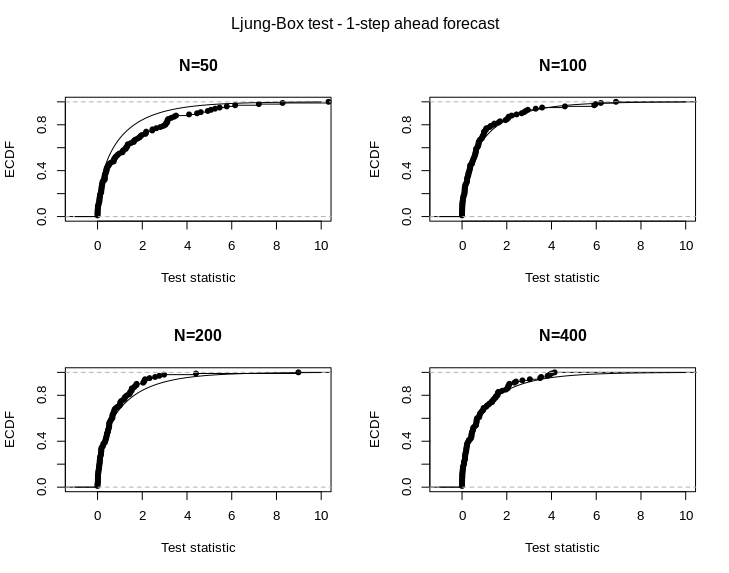
\includegraphics[width=14cm]{LB-1.png}
\caption{ECDF of the test statistic of the Ljung-Box test of independence, for 1-step ahead forecasting. The continuous line represents the true CDF under the null hypothesis.}
\label{fig:LB-1}
\end{figure}

\begin{figure}[ht]
\centering
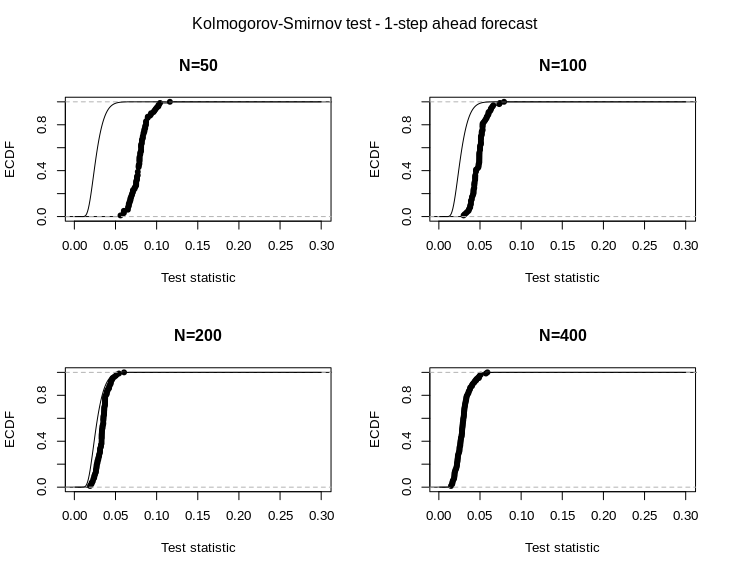
\includegraphics[width=14cm]{KS-1.png}
\caption{ECDF of the test statistic of the Kolmogorov-Smirnov test of uniformity, for 1-step ahead forecasting. The continuous line represents the true CDF under the null hypothesis.}
\label{fig:KS-1}
\end{figure}

\begin{figure}[ht]
\centering
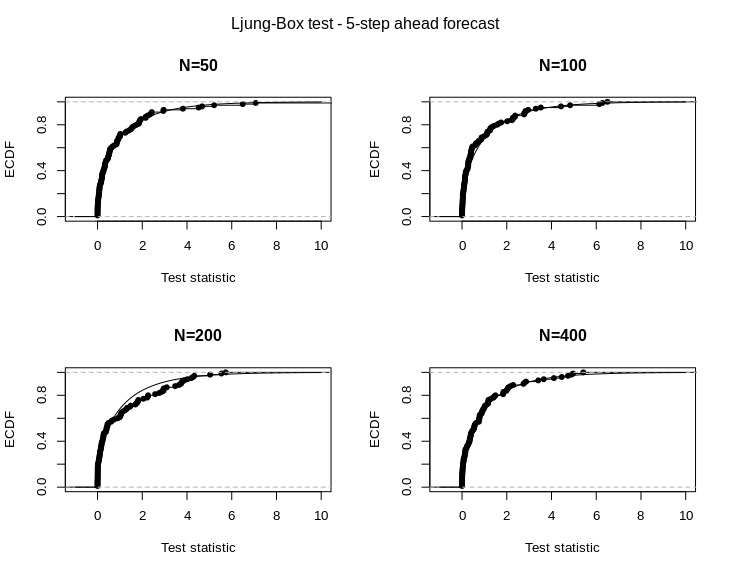
\includegraphics[width=14cm]{LB-5.png}
\caption{ECDF of the test statistic of the Ljung-Box test of independence, for 5-step ahead forecasting. The continuous line represents the true CDF under the null hypothesis.}
\label{fig:LB-5}
\end{figure}

\begin{figure}[ht]
\centering
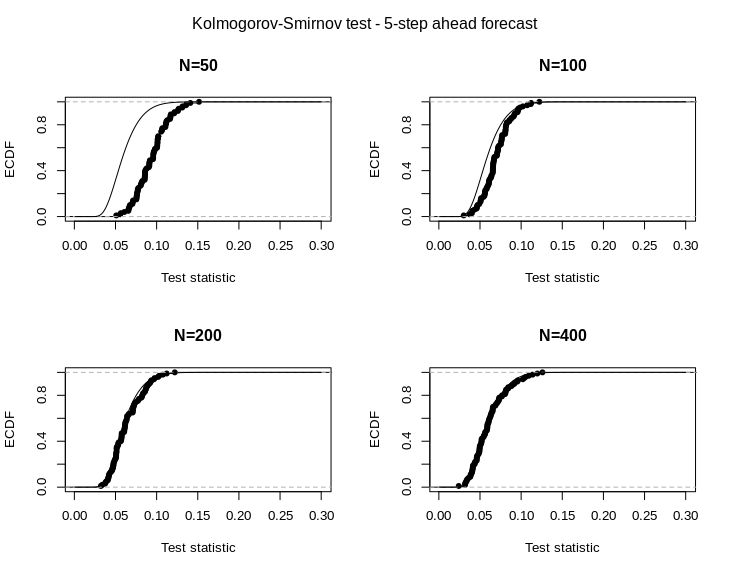
\includegraphics[width=14cm]{KS-5.png}
\caption{ECDF of the test statistic of the Kolmogorov-Smirnov test of uniformity, for 5-step ahead forecasting. The continuous line represents the true CDF under the null hypothesis.}
\label{fig:KS-5}
\end{figure}

Tables \ref{tab:LB} and \ref{tab:KS} show the average p-value of both tests over the 100 runs for different particle sample sizes $N$ and for 1-step ahead and 5-step ahead forecasting. The average p-values are observed to converge to 0.5 when $N$ increases, which is the expected value under the null hypothesis.

\begin{table}[ht]
\centering
\begin{tabular}{ |c|c|c|c| }
 \cline{3-4}
 \multicolumn{2}{c|}{} & \multicolumn{2}{c|}{$h$} \\
 \cline{3-4}
 \multicolumn{2}{c|}{} & $1$ & $5$ \\
 \hline
 \multirow{4}{*}{$N$} & $50$ & $0.41$ & $0.50$ \\ 
 & $100$ & $0.49$ & $0.53$ \\
 & $200$ & $0.51$ & $0.50$ \\ 
 & $400$ & $0.50$ & $0.50$ \\
 \hline
\end{tabular}
\caption{Average p-value of the Ljung-Box test of independence.}
\label{tab:LB}
\end{table}

\begin{table}[ht]
\centering
\begin{tabular}{ |c|c|c|c| }
 \cline{3-4}
 \multicolumn{2}{c|}{} & \multicolumn{2}{c|}{$h$} \\
 \cline{3-4}
 \multicolumn{2}{c|}{} & $1$ & $5$ \\
 \hline
 \multirow{4}{*}{$N$} & $50$ & $0.00$ & $0.11$ \\ 
 & $100$ & $0.04$ & $0.35$ \\
 & $200$ & $0.26$ & $0.46$ \\ 
 & $400$ & $0.44$ & $0.52$ \\
 \hline
\end{tabular}
\caption{Average p-value of the Kolmogorov-Smirnov test of uniformity.}
\label{tab:KS}
\end{table}

Thus, the null hypotheses of the Ljung-Box test of independence and the Kolmogorov-Smirnov test of uniformity tend to be more statistically likely when the number of particles increases. This empirically validates the converge of particle forecasting to the optimal forecast.

\section{Conclusion}

In this article, we propose a novel forecasting algorithm for state-space models, particle forecasting, which is an extension of particle filtering. We obtain convergence results, almost surely and in mean squared error, for particle forecasting and we review results for particle filtering. Simulations are run to illustrate the convergence of particle filtering, using performance assessment techniques based on probability integral transform and adapted to distributional forecasts.

An application example for particle forecasting is value-at-risk (VaR) forecasting in stochastic volatility (SV) models for financial risk management \cite{BuiQuang2018}. SV models are state-space models describing time series of financial asset returns. VaR is a measure of risk based on quantiles of forecasts, hence the importance of having distributional forecasts, from which quantiles can be extracted.

Particle forecasting produces converging Monte Carlo approximations of the optimal forecast when the model is known. In practice, when working with real datasets, model specification strongly impacts forecasting performance. Particle forecasting can yield arbitrarily small approximation error, but it does not address the modelling error between the true data-generating process and the model.

Besides, particle forecasting relies on the possibility to generate samples from the observation model. In some settings, the conditional distribution of observations given the hidden state is intractable, which has motivated the development of approximate Bayesian computation \cite{Jasra2012}. In this context, particle forecasting cannot be straightforwardly applied and requires some adjustments.

Issues to investigate include the application of particle forecasting to real problems, especially those necessitating forecasts in the form of distributions \cite{Gneiting2014}, like VaR forecasting. On the theoretical side, convergence in distribution of particle forecasting remains to be assessed, typically with a central limit theorem with closed-formed asymptotic variance, as it is already available for particle filtering \cite{Chopin2004}.

\section*{References}

\bibliography{refs}

\section*{Appendix}

\subsection{Proofs of Lemmas \ref{lem:cv_sampling} and \ref{lem:cv_sampling_l2}}
\label{sec:proof-sampling}

\begin{proof}[Proof of Lemma \ref{lem:cv_sampling}]
    $$\int \phi \, s^N(\nu^N(V_{1:N})) - \int \phi \, \nu = \int \phi \, s^N(\nu^N(V_{1:N})) - \int \phi \, \nu^N(V_{1:N}) + \int \phi \, \nu^N(V_{1:N}) - \int \phi \, \nu,$$
    where it is assumed that $\displaystyle \int \phi \, \nu^N(V_{1:N}) - \int \phi \, \nu \limN 0$ almost surely. Then one must prove that $\displaystyle \int \phi \, s^N(\nu^N(V_{1:N})) - \int \phi \, \nu^N(V_{1:N}) \limN 0$ almost surely.
    
    One has that
    $$\E[(\int \phi \, s^N (\nu^N(V_{1:N})) - \int \phi \, \nu^N(V_{1:N}))^4] = \E[\E[(\frac 1N \sum_{i=1}^N \phi(U^i) - \int \phi \, \nu^N(V_{1:N}))^4 \mid V_{1:N}]] $$
    where $U_1,\dots,U_N \mid V_{1:N} \simiid \nu^N(V_{1:N})$, so that
    \begin{align*}
      &\E[(\frac 1N \sum_{i=1}^N \phi(U_i) - \int \phi \, \nu^N(V_{1:N}))^4 \mid V_{1:N}] \\
      &= \frac{1}{N^4} \sum_i \E[(\phi(U_i) - \int \phi \, \nu^N(V_{1:N}))^4 \mid V_{1:N}] \\
      & \ \ \ + \frac{3}{N^4} \sum_{i \neq j} \E[(\phi(U_i) - \int \phi \, \nu^N(V_{1:N}))^2 \mid V_{1:N}] \E[(\phi(U_j) - \int \phi \, \nu^N(V_{1:N}))^2 \mid V_{1:N}] \\
      &\leq \frac{N (2 |\sup \phi|)^4}{N^4} + \frac{3 N(N-1) (2 |\sup \phi|)^4}{N^4} \\
      &\leq \frac{48 |\sup \phi|^4}{N^2}.
    \end{align*}
    Thus
    $$\E[(\int \phi \, s^N (\nu^N(V_{1:N})) - \int \phi \, \nu^N(V_{1:N}))^4] \leq \frac{48 |\sup \phi|^4}{N^2}. $$
    For all $\varepsilon>0$,
    \begin{align*}
        & \sum_{N=1}^{\infty} \prob [ |\int \phi \, s^N (\nu^N(V_{1:N})) - \int \phi \, \nu^N(V_{1:N})| \geq \varepsilon] \\
        &\leq \sum_{N=1}^\infty \frac{\E[(\int \phi \, s^N (\nu^N(V_{1:N})) - \int \phi \, \nu^N(V_{1:N}))^4]}{\varepsilon^4} \\
        &\leq \frac{48 |\sup \phi|^4}{\varepsilon^4}\sum_{N=1}^{\infty}\frac{1}{N^2} <\infty,
    \end{align*}
    by the Markov inequality. From the Borel-Cantelli lemma, one can conclude that
    $\displaystyle \int \phi \, s^N(\nu^N(V_{1:N})) - \int \phi \, \nu^N(V_{1:N}) \limN 0$ almost surely.
\end{proof}

\begin{proof}[Proof of Lemma \ref{lem:cv_sampling_l2}]
    One has that
    $$ \int \phi \, s^N(\nu^N(V_{1:N})) - \int \phi \, \nu = \int \phi \, s^N(\nu^N(V_{1:N})) - \int \phi \, \nu^N(V_{1:N}) + \int \phi \, \nu^N(V_{1:N}) - \int \phi \, \nu. $$
    According to the Minkowski inequality,
    \begin{multline*}
        \E[(\int \phi \, s^N(\nu^N(V_{1:N})) - \int \phi \, \nu)^2]^{1/2} \leq \E[(\int \phi \, s^N(\nu^N(V_{1:N})) - \int \phi \, \nu^N(V_{1:N}))^2]^{1/2} \\
        + \E[(\int \phi \, \nu^N(V_{1:N}) - \int \phi \, \nu)^2]^{1/2}
    \end{multline*}
    where it is assumed that $\displaystyle \E[(\int \phi \, \nu^N(V_{1:N}) - \int \phi \, \nu)^2]^{1/2} \leq \sqrt{\frac{m}{N}}$.
    
    Then
    $$ \E[(\int \phi \, s^N(\nu^N(V_{1:N})) - \int \phi \, \nu^N(V_{1:N}))^2] = \E[\E[(\int \phi \, s^N(\nu^N(V_{1:N})) - \int \phi \, \nu^N(V_{1:N}))^2 \mid V_{1:N}]]$$
    and
    \begin{align*}
        &\E[(\int \phi \, s^N(\nu^N(V_{1:N})) - \int \phi \, \nu^N(V_{1:N}))^2 \mid V_{1:N}] \\
        &= \E[(\frac 1N \sum_{i=1}^N \phi(U_i) - \int \phi \, \nu^N(V_{1:N}))^2 \mid V_{1:N}] \\
        &= \frac 1N (\int \phi^2 \, \nu^N(V_{1:N}) - (\int \phi \, \nu^N(V_{1:N}))^2) \\
        &\leq \frac{2 |\sup \phi|^2}{N}
    \end{align*}
    where $U_1,\dots,U_N \mid V_{1:N} \simiid \nu^N(V_{1:N})$, thus
    $$ \E[(\int \phi \, s^N(\nu^N(V_{1:N})) - \int \phi \, \nu^N(V_{1:N}))^2]^{1/2} \leq \frac{\sqrt 2 |\sup \phi|}{\sqrt N}. $$
\end{proof}

\subsection{Proofs of Propositions \ref{prop:pred_continuous}, \ref{prop:upd_continuous} and \ref{prop:for_continuous}}
\label{sec:proof-continuity}

\begin{proof}[Proof of Proposition \ref{prop:pred_continuous}]
    Let $\phi$ be a continuous bounded function. Let $\{\nu^N\}_N$ be a converging sequence of probability measures with limit $\nu$ in the weak topology. One has that
    \begin{align*}
        \int \phi \, \pred_t(\nu^N) &= \int \phi(x') [\int Q_t(x,dx') \, \nu^N(dx)] \\
        &= \int [\int \phi(x') Q_t(x,dx') ] \, \nu^N(dx) \\
        &\limN \int [\int \phi(x') Q_t(x,dx') ] \, \nu(dx)
        \intertext{as $\displaystyle \int \phi(x_t) Q_t(\cdot,dx_t)$ is continuous and bounded from Assumption \ref{assu:feller} and $\nu^N \limN \nu$}
    &= \int \phi(x') [\int Q_t(x,dx') \, \nu(dx)] \\
    &= \int \phi \, \pred_t(\nu).
  \end{align*}
\end{proof}

\begin{proof}[Proof of Proposition \ref{prop:upd_continuous}]
    Let $\phi$ be a continuous bounded function. Let $\{\nu^N\}_N$ be a converging sequence of probability measures with limit $\nu$ in the weak topology. One has that
    \begin{equation*}
       \int \phi \, \upd_t(\nu^N) = \frac{\int \phi(x) \, g_t(Y_t \mid x) \, \nu^N(dx) }{\int g_t(Y_t \mid x) \, \nu^N(dx)}. 
    \end{equation*}
    In this ratio, from Assumption \ref{assu:g_bounded}, the numerator verifies
    \begin{equation*}
        \int \phi(x) \, g_t(Y_t \mid x) \, \nu^N(dx) \limN \int \phi(x) \, g_t(Y_t \mid x) \, \nu(dx)    
    \end{equation*}
    because $\phi \, g$ is continuous and bounded and the denominator verifies
    \begin{equation*}
        \int g_t(Y_t \mid x) \, \nu^N(dx) \limN \int g_t(Y_t \mid x) \, \nu(dx) > 0  
    \end{equation*}
    because $g$ is continuous, bounded and strictly positive. As the limit of the denominator is nonzero, one has that
    \begin{equation*}
        \int \phi \, \upd_t(\nu^N) \limN \frac{\int \phi(x) \, g_t(Y_t \mid x) \, \nu(dx) }{\int g_t(Y_t \mid x) \, \nu(dx)} = \int \phi \, \upd_t(\nu).    
    \end{equation*}
\end{proof}

\begin{proof}[Proof of Proposition \ref{prop:for_continuous}]
    Let $\phi$ be a continuous bounded function. Let $\{\nu^N\}_N$ be a converging sequence of probability measures with limit $\nu$ in the weak topology. One has that
    \begin{equation*}
        \int \phi \, \for_t(\nu^N) = \int \phi(y) \, [\int g_t(y \mid x) \, \nu^N(dx)] \, \lambda(dy) = \int [\int \phi(y) \, g_t(y \mid x)\, \lambda(dy)] \, \nu^N(dx)
    \end{equation*}
    where $\displaystyle \int \phi(y) \, g_t(y \mid \cdot)\, \lambda(dy)$ is continuous from Assumption \ref{assu:varphi_continuous} and bounded by $\sup|\phi|$. Thus
    \begin{equation*}
        \int \phi \, \for_t(\nu^N) \limN \int [\int \phi(y) \, g_t(y \mid x)\, \lambda(dy)] \, \nu(dx)
    \end{equation*}
    where the limit equals $\displaystyle \int \phi(y) \, [\int g_t(y \mid x) \, \nu(dx)] \, \lambda(dy) = \int \phi \, \for_t(\nu)$.
\end{proof}

\subsection{Probability Integral Transform}
\label{sec:PIT}

Let $F_{t+h \mid t}$ be the cdf of the optimal forecast $f_{t+h \mid t}$, i.e.\ the conditional cdf of $Y_{t+h}$ given $Y_{0:t}$.

The PIT $F_{t+h \mid t}(Y_{t+h})$ is a random variable taking values in $[0,1]$ equipped with its Borelian set. One has that
\begin{equation*}
    \E[\phi(F_{t+h \mid t}(Y_{t+h})) \mid Y_{0:t}] = \int_0^1 (\phi \circ F_{t+h \mid t}) \, f_{t+h \mid t} = \int_0^1 \phi \, (f_{t+h \mid t} \circ F_{t+h \mid t}^{-1})    
\end{equation*}
where the pushforward measure $f_{t+h \mid t} \circ F_{t+h \mid t}^{-1}$ is the Lebesgue measure. Indeed, let $[a,b[ \subset [0,1]$ ($a<b$) and $a'$, $b' \in \mathbb R$ such that $F_{t+h \mid t}(a')=a$ and $F_{t+h \mid t}(b')=b$, then $f_{t+h \mid t}(F_{t+h \mid t}^{-1}([a,b[)) = f_{t+h \mid t}([a',b'[)=F_{t+h \mid t}(b') - F_{t+h \mid t}(a')=b-a$.

Thus $F_{t+h \mid t}(Y_{t+h})$ and $Y_{0:t}$ are independent and $F_{t+h \mid t}(Y_{t+h}) \sim \mathcal U(0,1)$.

\end{document}
